
\subsection{RVAgene can accurately and efficiently reconstruct temporal profiles from synthetic data}
We generated a dataset of 120 genes using convolutions of sinusoidal functions (see Methods) to test
the ability of RVAgene (\hyperref[fig:fig2]{fig. 6.1A}) to learn and reconstruct noisy nonlinear
temporal profiles. An RVAgene model was trained on all 120 genes from 6 clusters with a hidden size
of 70 and a 3 dimensional latent space. The model was trained for 400 epochs, after which the
average batch objective $\cL$ function indicates convergence (\hyperref[fig:fig2]{fig. 6.1B}),
producing a three-dimensional latent space representation (\hyperref[fig:fig2]{fig. 6.1C}). K-means
clustering on the latent space (k=6) identified well-separated clusters (\hyperref[fig:fig2]{fig. 6.1D}).
%Thus, RVAgene has learnt a latent space in which different temporal profiles can be readily identified and classified using simple clustering methods. 


{\centering
\begin{figure}
  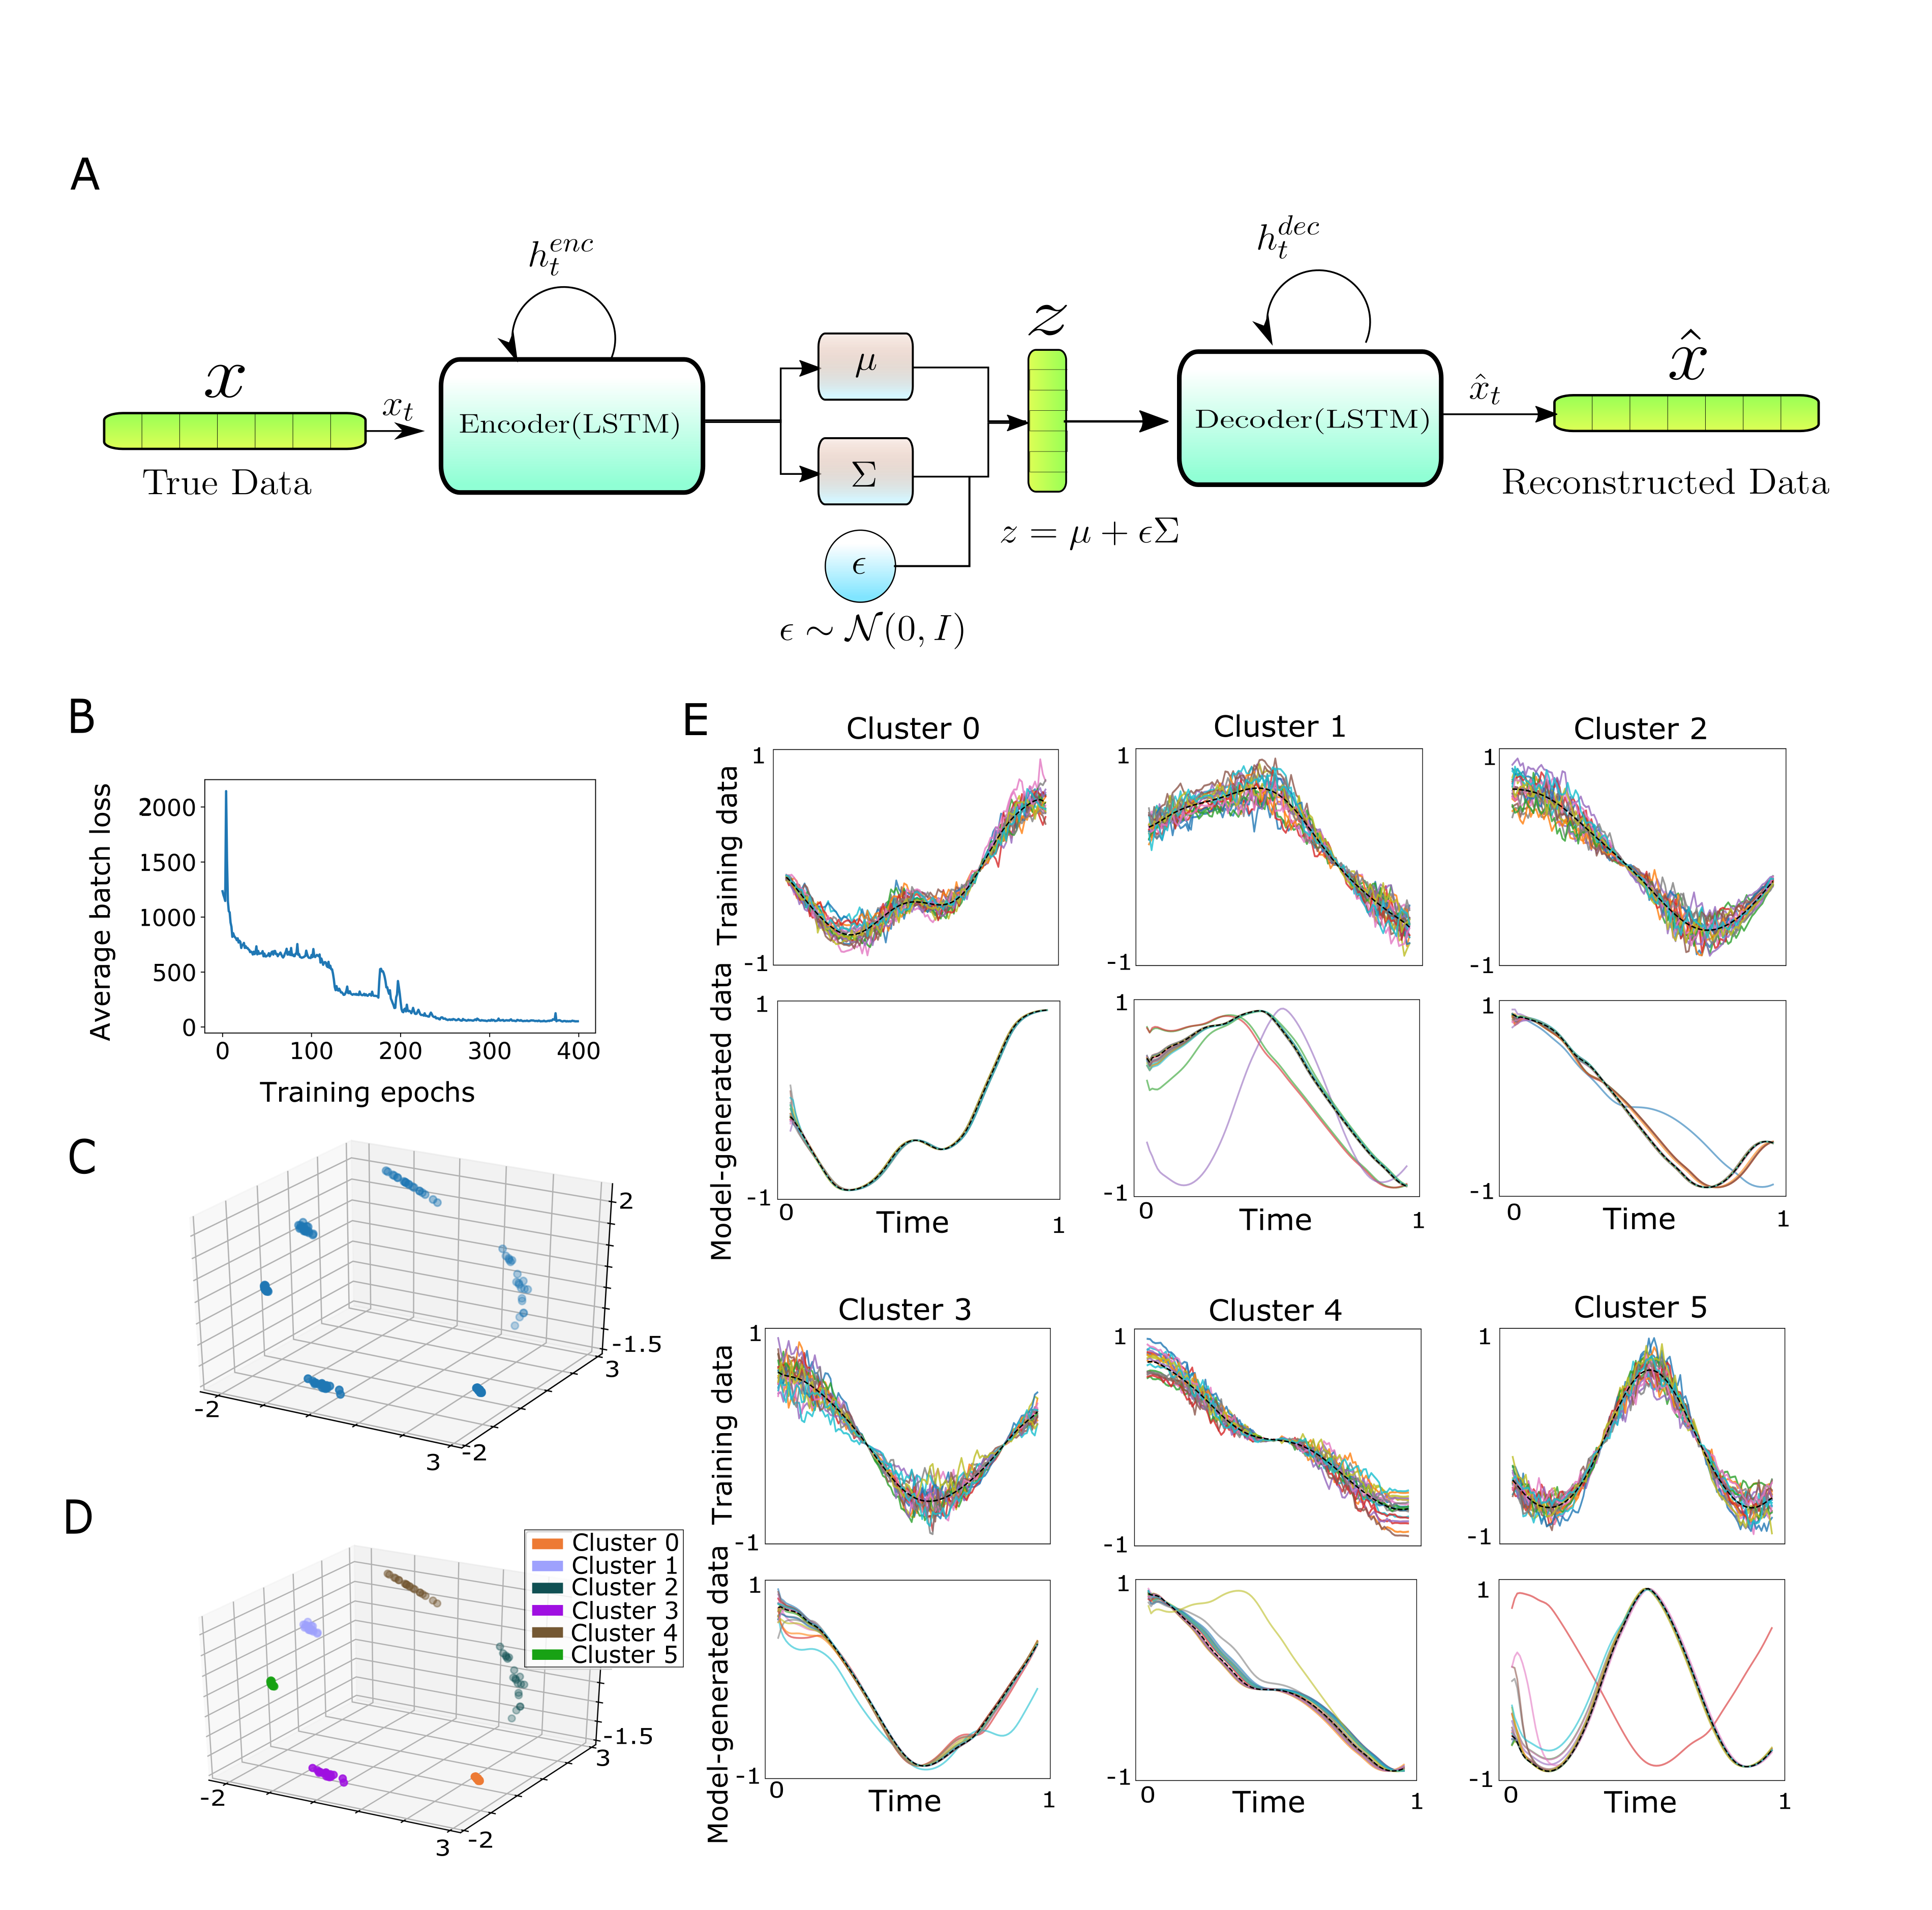
\includegraphics[width=\linewidth]{figures/fig2.png}
 % archetecture.png: 1149x508 px, 72dpi, 40.53x17.92 cm, bb=0 0 1149 508
    \caption[Unsupervised representation learning with RVAgene using synthetic data.]{\textbf{Unsupervised representation learning with RVAgene using synthetic data.} ({\bf A}) Schematic diagram of the RVAgene model. ({\bf B}) Average loss function $\cL$ as over duration of training.
    ({\bf C}) Latent space representation learnt by RVAgene model after training.
    ({\bf D}) Clusters detected by $k$-means clustering on the latent space, with $k=6$
    ({\bf E}) First and third rows show input training data used (20 simulated genes in each of six clusters); cluster means shown in black. Second and fourth rows show the model-generated data, obtained by sampling and decoding points from the latent space; decoded cluster empirical means shown in black.} 
 \label{fig:fig2}
\end{figure}
}
%%\tcr{I'm not sure about this in light of Svensson et al. we should discuss it.} 
RVAgene modeling followed by k-means clustering on the latent space identified 6 clusters with perfect fidelity between predicted and true clusters. One might reasonably ask, why use a neural network for this task? Simpler dimensionality reduction methods (e.g. PCA, t-SNE, or a non-variational autoencoder) would also find the correct solution. RVAgene has the advantage over these methods that the underlying structure of the latent space leads to interpretability. A point in reduced PCA or t-SNE space that does not overlap with a data point is not interpretable. Traditional autoencoders lack regularity in the latent space, i.e. even for a representation with arbitrary accuracy (a reconstruction error of zero), decoding a point that does not correspond to a training data point can result in nonsensical generated data, even if the decoded point is arbitrarily close to a training data point. Variational Auoencoders remedy this by learning a regularized or smoother distribution on the latent space. In this sense, the KL-divergence term in the VAE loss function can be thought of as a regularizer. This property enables RVAgene to generate new gene expression dynamics by decoding points from different regions of the latent space, having properties similar to clusters nearby to those points.


To demonstrate the generative properties of the RVAgene latent space, we sample points from
multivariate Normal distributions, centered on the empirical mean of each cluster with variance of
0.4, i.e. $\cN(\mu_c, 0.4I)$, where $\mu_c$ is the empirical mean of the cluster and $\vI$ is the
identity matrix in $\mathbb{R}^3$. Corresponding to each cluster, we sample 20 points in the latent
space, and use the decoder network to generate new time series data (\hyperref[fig:fig2]{fig. 6.1E}). Most of the points sampled generate trajectories that belong to the correct cluster. Moreover, we identify cases  corresponding to transitions between clusters. For example, some points sampled near Cluster 2 generate trajectories that are similar to members of Cluster 4, and vice versa. This makes sense due to the similarity between the temporal profiles of Clusters 2 and 4. A similar correspondence is observed between Clusters 1 and 5.
{We note that in a few cases the generated data have profiles that differ from their cluster of
origin and appear most similar to those of another cluster. This occurs when points are sampled
close to neighboring clusters, e.g. the red line for Cluster 5 in \hyperref[fig:fig2]{fig. 6.1E} has been sampled from a point close to cluster 3.}
We also observe some generated trajectories that display intermediate profiles between two or more clusters: the decoder function learnt by RVAgene is smooth, and gives rise to meaningful representations of points across regions of the latent space. 
\par
RVAgene offers additional functionality as a tool for removing noise from the data. Via sampling and
decoding points from the latent space, RVAgene reconstructs trajectories that are smooth and
de-noised relative to the input data (\hyperref[fig:fig2]{fig. 6.1E}, \hyperref[fig:figS1]{Fig. S16}). Similar neural network approaches have been proposed to denoise from single-cell data, e.g. using a deep count autoencoder \citep{eraslan2019single}. RVAgene provides data denoising as a by-product of its primary functionality: learning patterns of dynamic gene expression.
\par
{To investigate the impact of input noise levels on RVAgene performance, we added Gaussian noise
drawn from $\cN(0,0.7)$ to the simulated data to produce a dataset with higher overall noise levels.
RVAgene learns a latent space shown in (\hyperref[fig:figS1]{Fig. S16A}) from which six clusters are
identified by k-means clustering (\hyperref[fig:figS1]{Fig. S16B}). It is notable that the clusters
identified in the latent space are not as clear in this case as for lower noise levels
(\hyperref[fig:fig2]{fig. 6.1}), however RVAgene can still reconstruct the distinct profiles with high confidence. To illustrate this, we plot the original training data alongside model-generated data, sampled at random points in the latent space from  $\cN(\mu,0.4\bI)$ around each cluster mean $\mu$ for each of the 6 clusters (\hyperref[fig:figS1]{Fig. S16C}). From these simulations, RVAgene appears able to separate even relatively high levels of noise from the signal, in order to learn a smooth encoding and corresponding generative process for distinct temporal patterns.}

%Similar to other VAE-based tools for the analysis of single-cell data, RVAgene is efficient and scalable for use with large datasets. We compared the performance of RVAgene with a Bayesian nonparametric approach for the analysis of gene expression time series data (Dirichlet Process Gaussian Process \citep{McDowell2018}. Using either CPU or GPU computing, the time and memory gains are substantial, enabling the analysis of larger datasets than would otherwise be possible (\hyperref[supp]{Fig. S1}). Analysis of RVAgene using simulated temporal data highlights the ability of such an architecture as means to study and generate gene expression dynamics. It enables learning of an unsupervised representation space, on which post-processing (e.g. unsupervised clustering) can be performed, as well as data denoising, and the generation of new time series data from arbitrary points in the latent space.
\par
It is inevitably challenging to include sufficient dimensionality and variation in synthetic datasets to accurately capture biological processes such as those we observe in experimental datasets. Thus, in the subsequent two sections, we test the capabilities of RVAgene on two whole-genome biological datasets: embryonic stem cell differentiation, and kidney injury response. As we will see, in these cases it may not be possible to characterize the latent space by simple (e.g. k-means) clustering; we need to use other means to gain insight into the features of the latent space.


